\chapter{Analiza procesu}

\section{Ogólna charakterystyka}
Proces badany w  niniejszej pracy to linia montująca płyty drukowane do finalnych produktów.
Składa się on z następujących etapów:
\begin{enumerate}
	\item Pobranie potrzebnych elementów elektronicznych z magazynu.
	\item Uzbrojenie automatu pick\&place w wymagane elementy.
	\item Pobranie gotowych płyt PCB (ang. Printed Circuit Board).
	\item Ręczne nałożenie pasty lutowniczej za pomocą sitodruku.
	\item Uruchomienie procesu montażu elementów na maszynie pick\&place.
	\item Umieszczenie ręczne elementów (opcjonalnie).
	\item Przeprowadzenie procesu lutowania w piecu.
	\item Lutowanie ręczne (opcjonalnie).
	\item Kontrola gotowej płyty PCB\@.
\end{enumerate}

\breakparagraph{}
Specyfika procesu:
\begin{itemize}
	\item wszystkie procedury muszą być wykonane w ustalonej kolejności,
	\item proces wymaga operatorów,
	\item dla płyt dwustronnych należy powtórzyć sekwencję,
	\item automat pick\&place może obsługiwać tylko jedną płytę PCB,
	\item piec lutowniczy może lutować kilka płyt drukowanych (ilość jest zależna od rozmiaru płyt).
\end{itemize}

Cały przepływ pracy został przedstawiony przy pomocy diagramu na Rysunku~\ref{DiagFlow}.
Czerwone krawędzie wyznaczają ścieżkę krytyczną procesu.
Węzły o krawędziach przerywanych są to operacje opcjonalne zależne od projektu płyty PCB\@.

\begin{figure}[H]
	\centering
	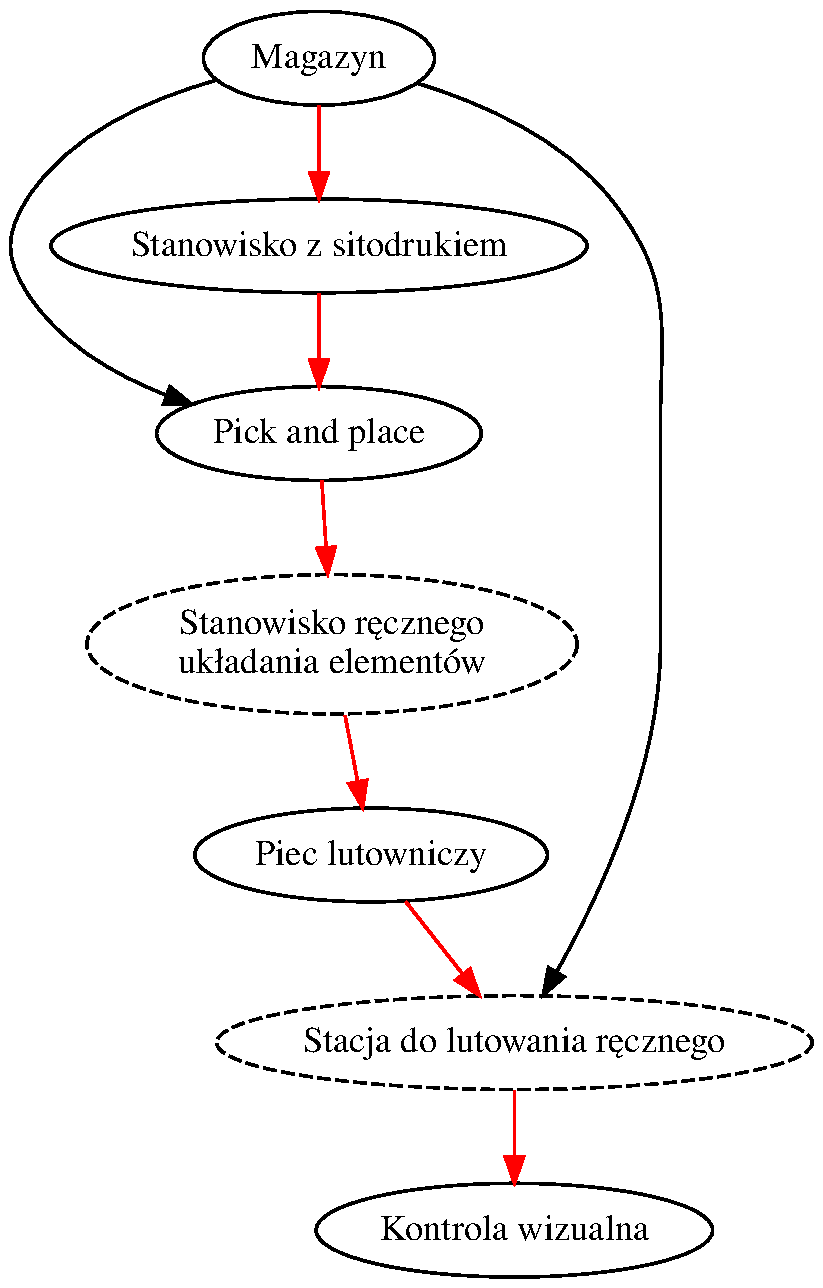
\includegraphics[scale=0.5]{./chapters/chapter2/flow_work.pdf}
	\caption{Diagram przepływu pracy w procesie}
	\label{DiagFlow}
\end{figure}

\section{Opis stanowisk}

\subsection{Magazyn}
Magazyn jest miejscem od, którego zaczyna się cały proces.
Przechowuje on wszystkie niezbędne elementy elektroniczne (rezystory, kondensatory, układy scalone itd.), gotowe płyty PCB oraz szablony sitodruku do poszczególnych projektów.
Aktualny stan magazynowy oraz fizyczna lokalizacja produktów znajduję się w systemie ERP\@.
Wszystkie potrzebne przedmioty są pobierane przez operatora.

\subsection{Stanowisko z sitodrukiem}
W kolejnym etapie produkcji gotowa płytka PCB trafia na urządzenie sitodruku.

(Opisać czym jest maszyna sitodruku)

Możemy wyszczególnić kilka typów takiej maszyny~\cite{sitodruk}:
\begin{itemize}
	\item sitodruk manualny --- najprostsza wersja urządzenia. Cały proces sprowadza się do ręcznego ustawienia szablonu na płytce oraz ręcznego nałożenia pasty przez operatora. Cechuję się gorszą jakością i powtarzalnością operacji w porównaniu do urządzeń przedstawionych poniżej.
	\item sitodruk półautomatyczny --- operator ustawia płytkę względem szablonu zazwyczaj przy pomocy systemu wizyjnego. Proces naniesienia pasty odbywa się automatycznie. Rozwiązanie to często wykorzystuje się przy prototypowaniu oraz produkcji małoseryjnej.
	\item sitodruk automatyczny --- rola operatora sprowadza się do podania płytki i odebrania po naniesieniu pasty (system offline) lub załadowania podajnika czystymi płytkami i później odebraniu gotowych (rozwiązanie in-line). Wszystkie czynności takie jak ustawienie szablonu i nałożenie pasty odbywają się automatycznie.
\end{itemize}

W analizowanym przypadku używany jest sitodruk manualny (Rysunek~\ref{sitodruk}). Operator przed nałożeniem pasty na płytę PCB musi przezbroić maszynę. Proceder polega na przyniesieniu szablonu z magazynu oraz ustawieniu go na maszynie. W dalszym kroku następuje manualne naniesienie pasty.

\begin{figure}[H]
	\centering
	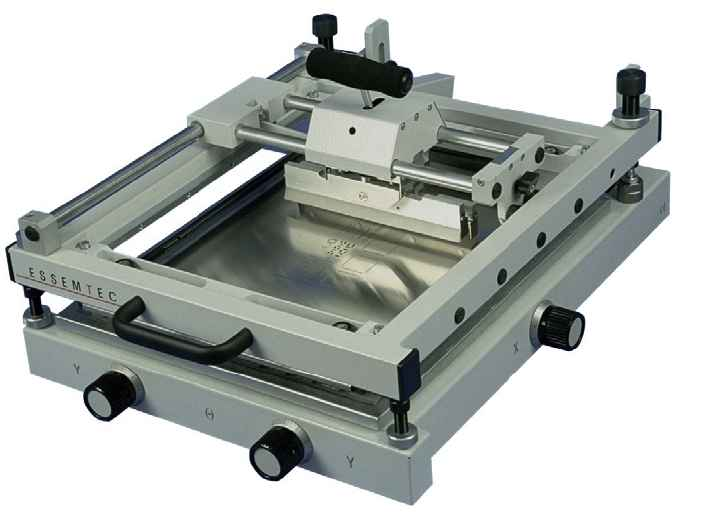
\includegraphics[scale=0.25]{./chapters/chapter2/sitodruk.jpg}
	\caption{Urządzenie sitodruku manualnego~\cite{sitodruk}}
	\label{sitodruk}
\end{figure}

\subsection{Automat pick\&place}
Automat pick and place to maszyna, która umożliwia w precyzyjny sposób układać komponenty SMD na płytkach PCB za pomocą systemu wizyjnego~\cite{automatp&p1}. W badanym procesie wykorzystywany jest automat M10V firmy Mechatronika (Rysunek~\ref{automat_pick_place}). Średnia wydajność maszyny to około 1200 --- 1600 komponentów na godzinę.

\breakparagraph{}
Cechy maszyny~\cite{automatp&p2}:
\begin{itemize}
	\item wbudowany system wizyjny,
	\item pełna automatyzacja nanoszenia elementów na płytę drukowaną,
	\item automatyczna korekcja na podstawie znaczników (ang.\ fiducials),
	\item korygowanie elementów na podstawie wykrycia złych oznaczeń na płycie,
	\item automatyczna zmiana dysz,
	\item automatyczne podawanie luźnych elementów (po wcześniejszej kalibracji),
	\item dane mogą pochodzić z różnych systemów danych CAD lub być wprowadzane ręcznie w trybie TEACH-IN\@.
\end{itemize}

\newpage
Maszynę przed pracą z płytą PCB należy przezbroić. Operacja przezbrojenia polega na załadowaniu odpowiednich elementów elektronicznych oraz wykonaniu kalibracji.

\breakparagraph{}
Możliwe formy dostarczenia elementów do automatu:
\begin{itemize}
	\item taśmy 8 mm, 12 mm, 16 mm, 24 mm, 32 mm, 44 mm,
	\item tacki JEDEC,
	\item tuby SO8–PLCC84,
	\item elementy luzem.
\end{itemize}

\begin{figure}[H]
	\centering
	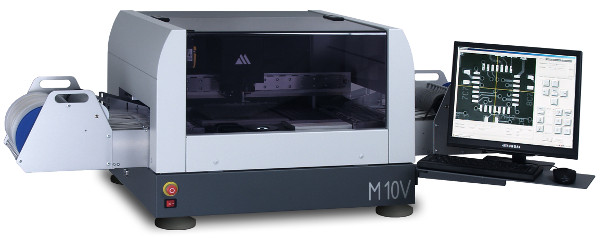
\includegraphics[scale=0.45]{./chapters/chapter2/M10V.jpeg}
	\caption{Automat M10V~\cite{automatp&p2}}
	\label{automat_pick_place}
\end{figure}


\subsection{Piec lutowniczy}
Piec lutowniczy to maszyna, która umożliwia zastosowanie w procesie techniki lutowania rozpływowego elementów SMD\@. Ważnym zagadnieniem przy lutowaniu rozpyłowym jest profil termiczny. Na podstawie profilu szacujemy czas trwania operacji na piecu.

\breakparagraph{}
Profil termiczny został schematycznie przedstawiony na Rysunku~\ref{schemat_termiczny} i składa się z następujących etapów:
\begin{description}
	\item[Etap 1] Nagrzewanie wstępne (preheat) --- wstępne nagrzewanie to jednostajny wzrost temperatury w tęmpie 1--3 \degree{C} do osiągnięcia około 150 \degree{C}. W tej fazie następuje częściowe odparowanie topnika.
	\item[Etap 2] Oczyszczanie (soak) --- aktywacja topnika umożliwiająca oczyszczenie chemiczne powierzchni złącza oraz usunięcie tlenków ze stopu lutowniczego. Etap ten trwa od 60 do 120 sekund.
	\item[Etap 3] Jednostajne rozgrzanie do rozpływu (ramp to peak) --- szybkie rozgrzanie mające na celu osiągnięcia temperatury likwidusu (temperatura przemiany ciała stałego w stan ciekły) stopu lutowniczego.
	\item[Etap 4] Rozpływ (reflow) --- faza zasadnicza lutowania rozpływowego. Zachodzi w temperaturze od 215 do 250 \degree{C} (zależne od użytego stopu lutowniczego). Na tym etapie płynny stop tworzy połączenie pomiędzy polem lutowniczym a elementem elektronicznym. Czas trwania rozpływu to od 30 do 300 sekund.
	\item[Etap 5] Chłodzenie (cooling) --- ostatni etap polegający na możliwe szybkim schłodzeniu o jednostajnym spadku 3--4 \degree{C}. Zbyt gwałtowne schłodzenie może spowodować naprężenie termiczne groźne dla elementów.
\end{description}

\begin{figure}[H]
	\centering
	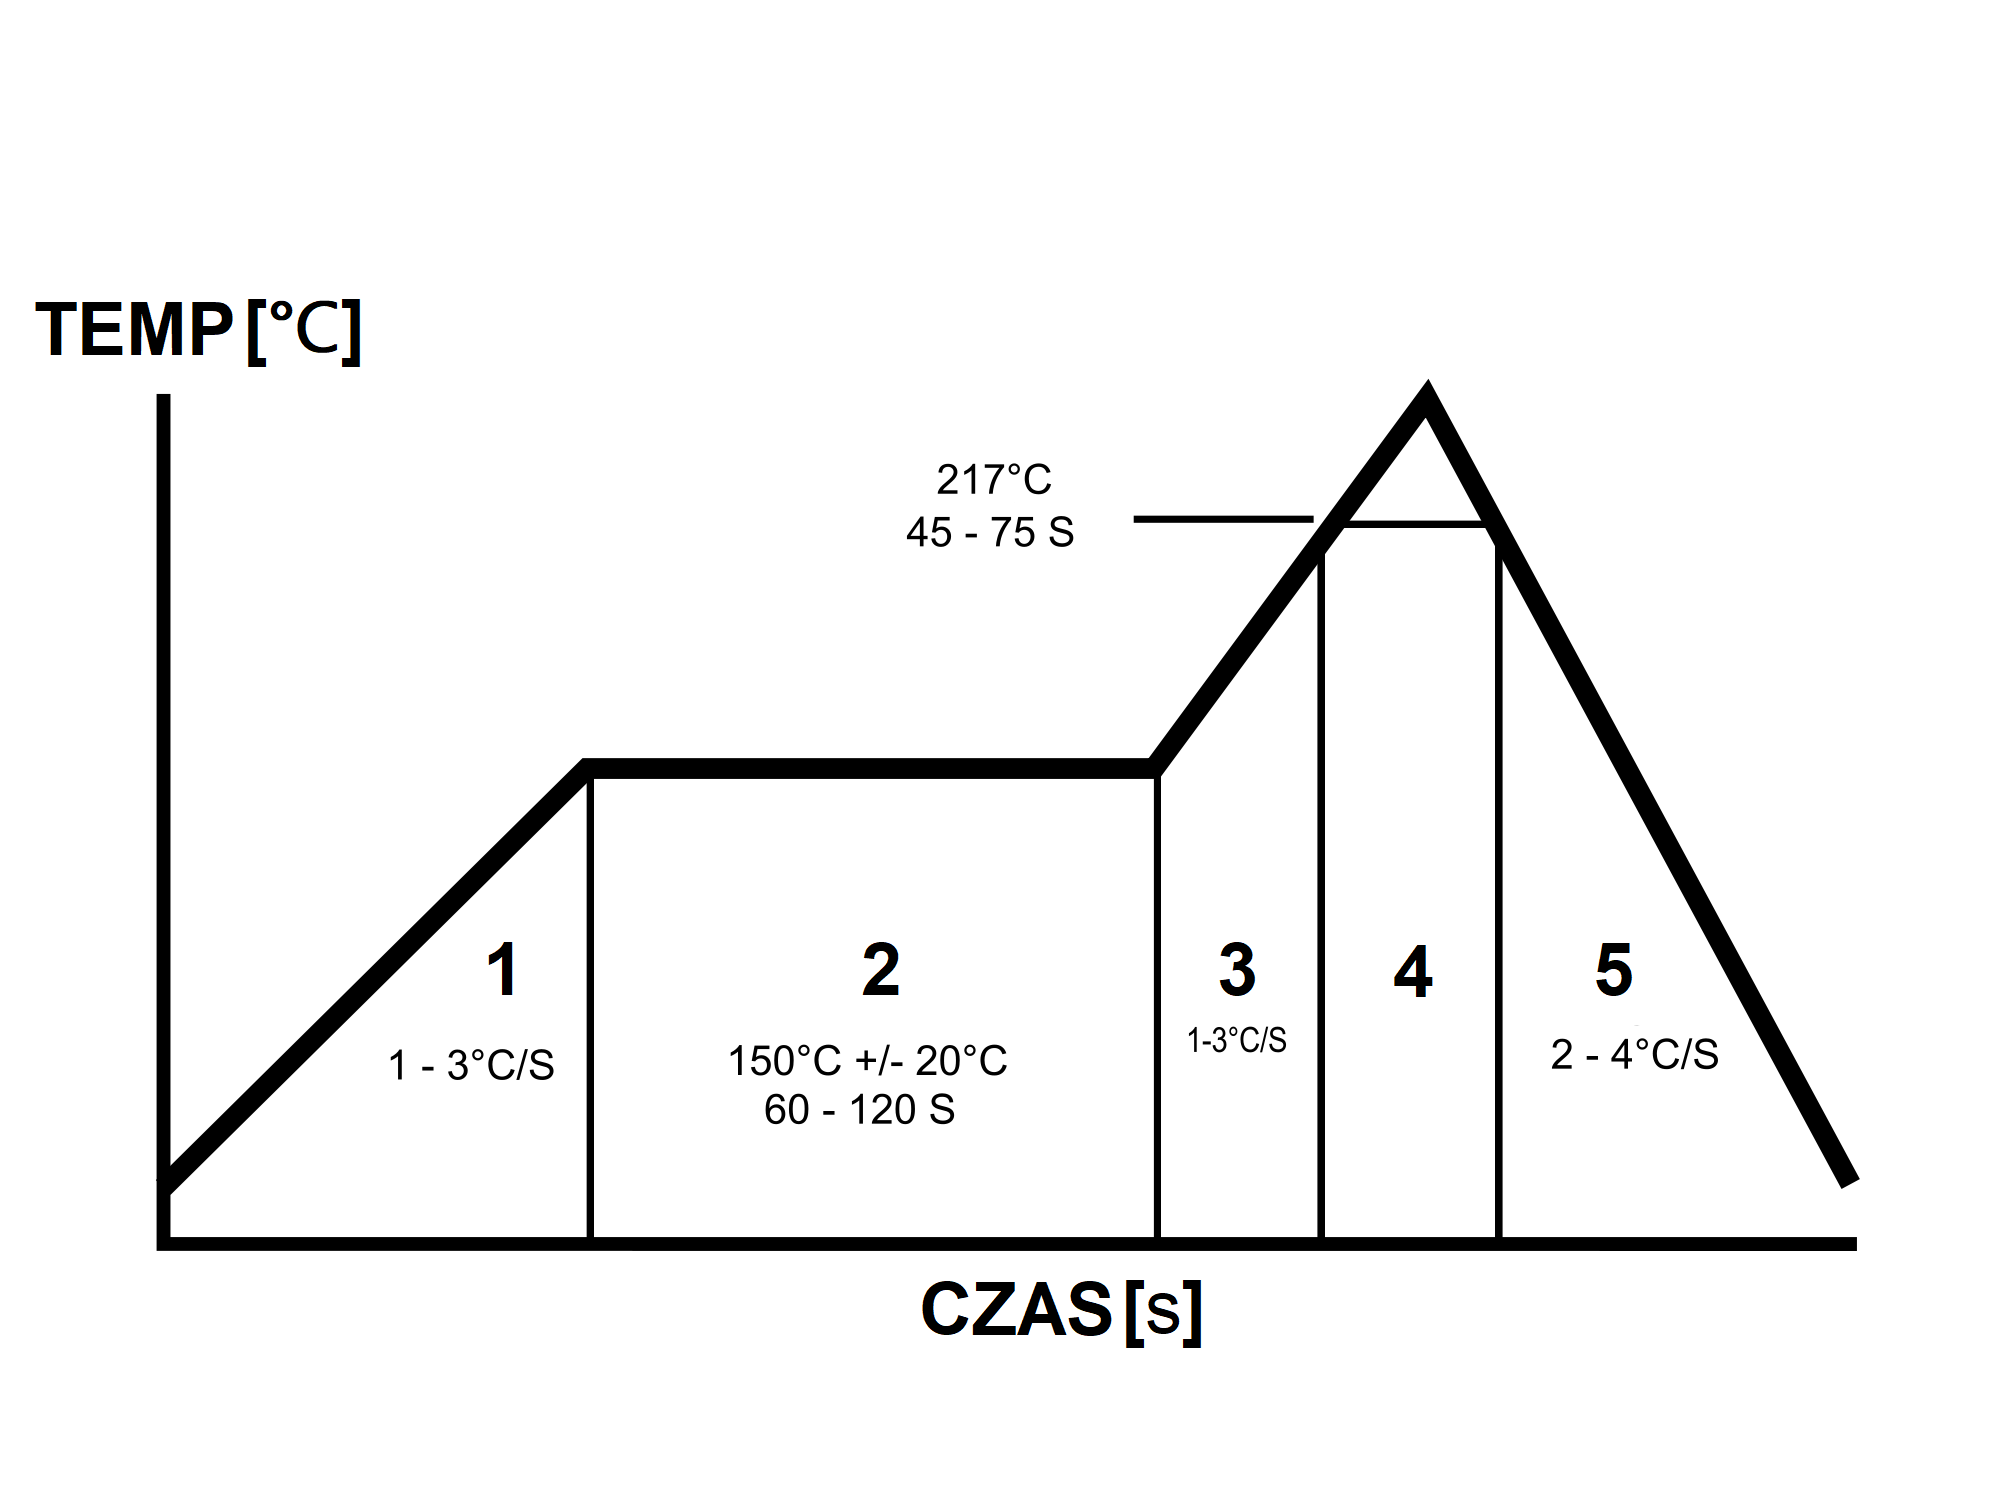
\includegraphics[scale=0.2]{./chapters/chapter2/schemat.png}
	\caption{Przebieg profilu termicznego w lutowaniu rozpływowym}
	\label{schemat_termiczny}
\end{figure}

W procesie jest wykorzystywany piec eC-reflow-mate firmy Eurocircuits (Rysunek~\ref{piec}).


\begin{table}[H]
	\centering
	\caption{Specyfikacja pieca}
	\begin{tabular}{cc}
		\toprule
		Maksymalny rozmiar płyty PCB & 350 $\times$ 250 mm              \\\midrule
		% Metody grzania                & promieniowanie IR, gorące powietrze \\\midrule
		Zakres temperatur             & Do 288 \degree{C}                \\\midrule
		Komunikacja z komputerem      & USB                              \\\midrule
		Wymiary                       & 520 $\times$ 620 $\times$ 245 mm \\\midrule
		Waga                          & około 25 kg                     \\
		\bottomrule
	\end{tabular}
\end{table}

\begin{figure}[H]
	\centering
	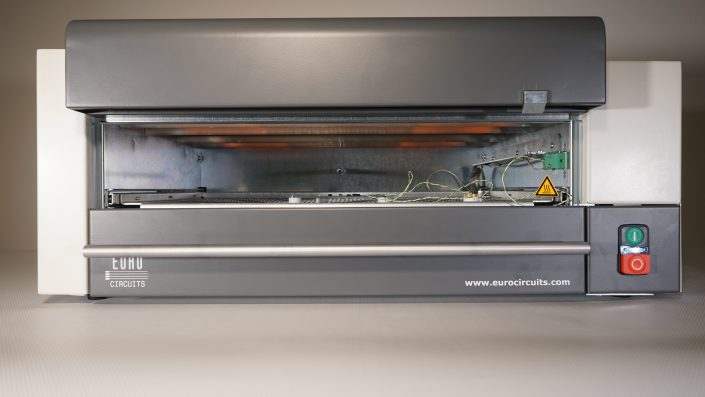
\includegraphics[scale=0.5]{./chapters/chapter2/piec.jpg}
	\caption{Piec lutowniczy eC-reflow-mate~\cite{piec}}
	\label{piec}
\end{figure}

\subsection{Stanowisko do prac ręcznych}
Operacje przeprowadzane przez operatora na tym stanowisku to ręczne nakładanie i lutowanie elementów oraz kontrola wizyjna.

\breakparagraph{}
Jest ono wyposażone w następujący sprzęt:
\begin{itemize}
	\item stację lutowniczą,
	\item stację hot-air,
	\item narzędzia drobne (szczypce, pęsety itd.),
	\item uchwyty montażowe,
	\item mikroskop.
\end{itemize}
